\documentclass[a4paper]{article}

\usepackage[spanish]{babel}
\usepackage{listings}
\usepackage[utf8]{inputenc}
\usepackage{titling}
\usepackage{enumitem}
\usepackage{fancyhdr}
\usepackage{xcolor}
\usepackage{geometry}
\usepackage{graphicx}
\usepackage{hyperref}
\geometry{a4paper, margin=7em}


\lstset{
    frame=single,
    breaklines=true,
    numbers=left,
    keywordstyle=\color{blue},
    numbersep=15pt,
    numberstyle=,
    basicstyle=\linespread{1.5}\selectfont\ttfamily,
    commentstyle=\color{gray},
    stringstyle=\color{orange},
    identifierstyle=\color{green!40!black},
}

%%\setlength{\parindent}{4em}
\setlength{\parindent}{0em}
\setlength{\parskip}{0.8em}
    
%%\renewcommand{\familydefault}{phv} %%Seleccionamos Helvetica
    
\lstdefinestyle{console}
{
    numbers=left,
    backgroundcolor=\color{violet},
    %%belowcaptionskip=1\baselineskip,
    breaklines=true,
    %%xleftmargin=\parindent,
    %%showstringspaces=false,
    basicstyle=\footnotesize\ttfamily,
    %%keywordstyle=\bfseries\color{green!40!black},
    %%commentstyle=\itshape\color{green},
    %%identifierstyle=\color{blue},
    %%stringstyle=\color{orange},
    basicstyle=\scriptsize\color{white}\ttfamily,
}
    
\title{Mapa de memoria}
\author{Aldán Creo Mariño}
    
    
\pagestyle{fancy}
\fancyfoot[R]{\thepage}
\fancyfoot[C]{}
\makeatletter
\let\runauthor\@author
\let\runtitle\@title
\makeatother
\fancyhead[L]{\runauthor}
\fancyhead[C]{SOI}
\fancyhead[R]{Práctica 5}
    
\begin{document}
%%\maketitle

\section{Mapa de memoria}

\subsection{Comentario previo}

Cada proceso en un sistema operativo moderno con multitarea se ejecuta en su propio \emph{contenedor}. Esto es lo que llamamos \emph{memoria virtual}. Esta memoria virtual se divide en páginas del mismo tamaño, y se incorporan a las páginas de memoria física a través de los registros de las tablas de páginas. Esta tabla la maneja el \emph{kernel}, y la consulta el procesador para saber dónde tiene que efectuar las operaciones. Cada proceso, como tiene su propia memoria virtual, tiene su propia tabla de páginas. Eso sí, no toda la memoria virtual va a estar al mismo tiempo en la memoria física (de ahí la necesidad de mantener un registro de qué páginas están y cuáles no).

La memoria virtual se divide en el espacio de usuario y el de kernel. En Linux, las únicas páginas que siempre van a estar presentes pertenecen al kernel, y son compartidas por todos los procesos (siempre están en la misma posición). Lo que ocurre, por tanto, cuando cambiamos de contexto, es un cambio de algunas páginas del espacio de usuario, pero no de las del núcleo. El mapa de memoria nos permite ver para un proceso los segmentos del espacio de memoria virtual que hemos reservado para un propósito determinado, y a lo largo de este informe comentaré los aspectos más relevantes de lo que podemos ver en este mapa.

\subsection{Mapa de memoria del ejercicio 6}

El siguiente mapa de memoria se produce cuando enlazo dinámicamente\footnote{Estoy usando {\ttfamily cat} para visualizar el contenido de {\ttfamily /proc/\$PID\$/maps} porque es el método sugerido, pero también se puede acceder al mapa de memoria usando {\ttfamily pmap}.}:

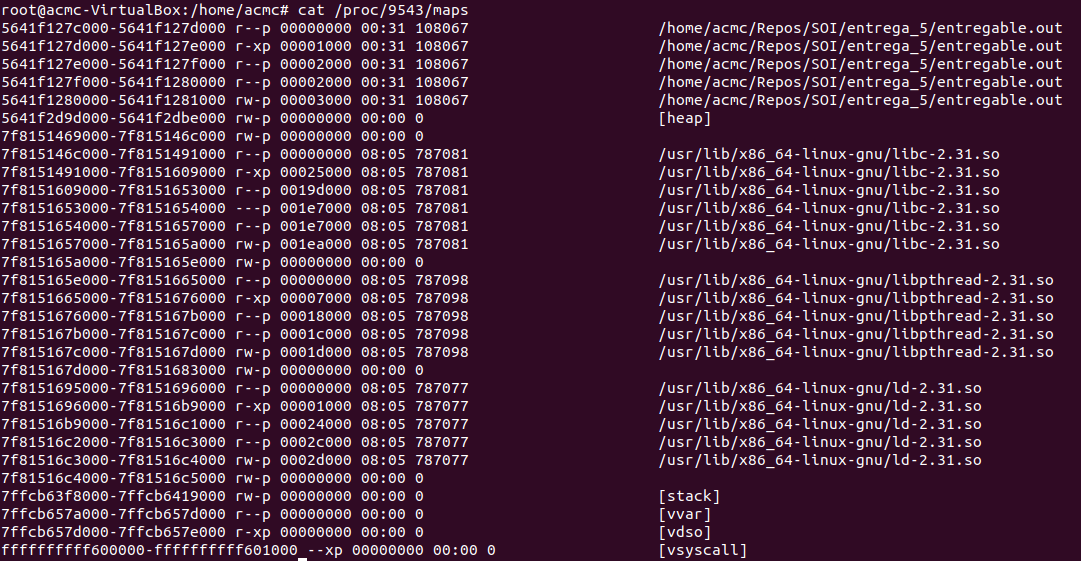
\includegraphics[scale=0.421]{6_padre.png}

Voy a comentar brevemente el significado de cada columna:

\begin{itemize}
    \item La primera columna se refiere a las direcciones de inicio y fin de la región de cada entrada del mapa. Están alineadas, en mi sistema, a los 4096 bytes (de ahí que, en hexadecimal, aparezcan alineadas a los {\ttfamily 0x1000} bytes). Excepto {\ttfamily [vsyscall]} (hablo sobre ella al final), todas están en la región de usuario.
    \item La segunda columna se refiere a los permisos que tenemos sobre ese segmento. Sobre esto hablaré en detalle más adelante, pero por ahora me limitaré a decir que {\ttfamily r} es para lectura, {\ttfamily w}, para escritura, y {\ttfamily x} para permitir la ejecución. La {\ttfamily p} se refiere a que es un segmento privado (no lo compartimos con otros procesos). Eso es lógico, ya que no queremos compartir ningún segmento de memoria con otro(s). Para no ser redundante, no haré más referencias a esto durante mi informe, pero es relevante comentarlo, ya que podría interesar que haya secciones \emph{shared}, en determinados casos de uso.
    \item La tercera columna es el desplazamiento dentro del archivo: si hemos mapeado ese segmento desde un archivo, entonces aquí indicamos el posible \emph{offset} que aplicamos dentro del mismo. Creo que esto se entiende sin mayor explicación.
    \item La cuarta columna, se refiere al número mayor y menor de dispositivo. Linux utiliza estos números para identificar los dispositivos (tanto físicos como virtuales), del sistema. El primero se refiere al driver, y el segundo, le sirve al driver para identificar el dispositivo específico.
    \item La quinta columna es el inodo, que identifica de forma única al fichero mapeado a memoria.
    \item Finalmente, la última columna, es el nombre del fichero, o nombres especiales como {\ttfamily [stack]}, o {\ttfamily [heap]}. Las entradas que no tienen nombre son ``regiones anónimas''.
\end{itemize}

\subsection{El segmento de texto}

El segmento de texto ({\ttfamily .text}), es el que contiene el código ejecutable del programa. En el mapa de memoria, es la entrada que tiene permisos de lectura y ejecución, y está mapeada al ejecutable (línea 2). Si imprimimos las direcciones de funciones, como por ejemplo hacemos en el ejercicio 2, veremos direcciones que corresponden a esa región de la memoria.

\subsection{Variables globales}

Las variables globales se guardan en el segmento de datos ({\ttfamily.data}, si están inicializadas, o si no, en {\ttfamily.bss})\footnote{Como se indica \href{https://stackoverflow.com/questions/8938303/how-to-get-the-data-and-bss-address-space-in-run-time-in-unix-c-program}{aquí}, dos segmentos pueden estar en la misma región.}. En el mapa de memoria del proceso, corresponderán con la sección con permisos de lectura y escritura, pero no ejecución, que se mapea al archivo del código (línea 5). En mi caso, el segmento de datos sin inicializar no contiene nada (no declaro variables sin inicializar).

Los \emph{vectores} son simplemente una secuencia de bytes, tal que $n_{bytes}=bytes_{elemento}*n_{elementos}$. No tienen nada especial.

\subsection{Variables locales}

Las variables locales se guardan en el stack. Cuando se entra en una función, el compilador de C incluye código para decrementar el \emph{stack pointer}, y guardar en el espacio que se ``crea'' (no en el mapa de memoria, sino que me refiero al espacio que queda libre al decrementar el puntero) las variables locales. Cuando se sale de la función, se incrementa el puntero, ``liberando'' en cierto modo la memoria.

Esto, en el mapa de procesos, se encuentra en la zona que se denota con la etiqueta {\ttfamily [stack]} (zona elevada de memoria, aunque la dirección exacta es aleatoria\footnote{Esto es así por cuestiones de seguridad: se evita que la posición en memoria de las secciones del programa se pueda conocer a priori. Más sobre esta cuestión en \href{https://manybutfinite.com/post/anatomy-of-a-program-in-memory/}{este artículo}.}). Lógicamente, tiene permisos {\ttfamily rw-p}. Podemos leer y escribir, pero no ejecutar, en esa zona.

El stack es el único segmento de memoria en el que, si se produce una referencia a memoria que no está dentro del segmento, pero sí dentro de su máximo total (usualmente unos 8MB), el sistema incrementa automáticamente su tamaño, en vez de lanzar un fallo de segmento (el comportamiento normal)\footnote{Como se indica en \href{https://stackoverflow.com/questions/54564273/dynamic-expansion-of-the-linux-stack}{este enlace}, el kernel decide si lanzar un fallo de segmento o aumentar el tamaño de este segmento comprobando el valor actual del \emph{stack pointer}.}. Esto es para permitir el crecimiento natural del {\ttfamily stack} con las llamadas a rutinas.

\subsection{Memoria dinámica}

La memoria dinámica es un concepto algo más complejo. Voy a hablar de las funciones de la familia {\ttfamily malloc}, aunque siendo estrictos podríamos gestionar la memoria dinámica nosotros mismos.

La gestión de la memoria se basa en el mapeo de direcciones de memoria arbitrariamente grandes a segmentos con permisos de lectura y escritura. Es decir, se trata de pedir al sistema regiones de memoria en las que poder trabajar con datos. {\ttfamily malloc} implementa esta idea a través de dos vías:

\begin{center}
    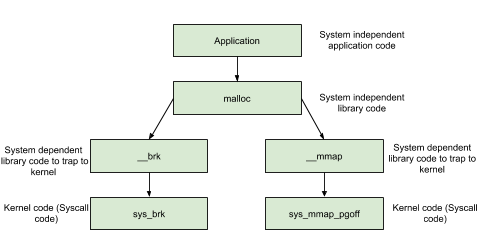
\includegraphics[scale=0.6]{malloc.png}\footnote{Imagen disponible \href{https://sploitfun.wordpress.com/2015/02/11/syscalls-used-by-malloc/}{en este artículo}.}
\end{center}


\begin{itemize}
    \item Usando memoria del {\ttfamily heap}. Si la memoria que le pedimos a {\ttfamily malloc} es relativamente pequeña, llegará con aumentar el tamaño del {\ttfamily heap} con la llamada al sistema {\ttfamily brk}.
    \item Si el tamaño que pedimos a {\ttfamily malloc}, en cambio, es mayor que {\ttfamily MMAP\_THRESHOLD} (valor configurable con la función {\ttfamily mallopt}), entonces {\ttfamily malloc} usa la llamada al sistema {\ttfamily mmap}, para crear un nuevo segmento en el que podamos leer y escribir.
\end{itemize}

Internamente, {\ttfamily malloc} lleva el control de las zonas de memoria que están libres para ofrecer al usuario y las que no, usando ``chunks'', disponibles en varios tamaños. Estos ``chunks'' son unidades de memoria que {\ttfamily malloc} asigna atómicamente: es decir, cuando solicitamos a {\ttfamily malloc} X bytes de memoria, nos devolverá una dirección dentro de un chunk libre, donde quepan esos X bytes, redondeados al siguiente tamaño posible de chunk (por ejemplo, si pido 500 bytes, y tengo de tamaños 256 y 512 bytes, entonces me devolverá un chunk de 512 bytes).\footnote{\href{https://danluu.com/malloc-tutorial/}{Aquí se explica} en mucho más detalle el funcionamiento de {\ttfamily malloc}. Es una lectura muy recomendada, porque el autor desarrolla una versión propia de un sistema de gestión de memoria dinámica equivalente al propio {\ttfamily malloc}.}.

Los chunks no son zonas de memoria totalmente vacías. Fijémonos en la siguiente imagen:
\begin{center}
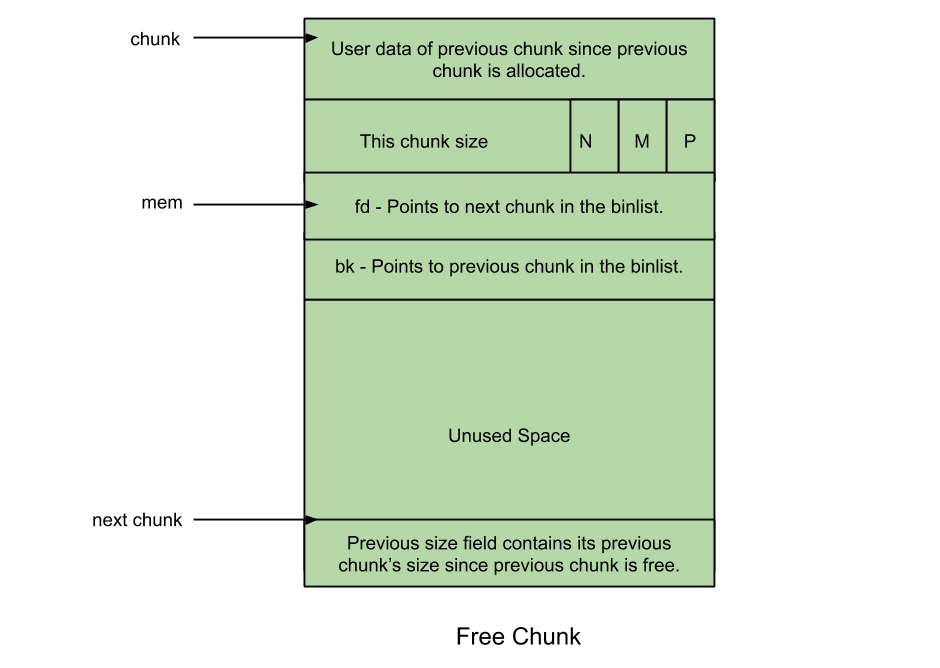
\includegraphics[scale=0.30]{Free_chunk.png}
\end{center}

Lo que podemos ver es que internamente {\ttfamily malloc} divide las zonas de memoria que usa en chunks, y guarda la información sobre el estado de cada chunk en el propio chunk. Además, los chunks siguen una estructura de lista enlazada: cada chunk apunta al siguiente. Además, en los casos de los chunks libres (el de la imagen), incluyen punteros al siguiente chunk libre y también al anterior (por lo que los chunks libres están al mismo tiempo en una lista doblemente enlazada). Esto le permite a {\ttfamily malloc} encontrar rápidamente un chunk libre en la memoria para ofrecérnoslo, y al mismo tiempo es el motivo de que ocurran carreras críticas en la implementación de {\ttfamily dlmalloc}, de la que hablaré más adelante. Pero la idea es que cuando tenemos varios hilos que intentan buscar al mismo tiempo un chunk libre, es una carrera crítica porque al encontrar el chunk libre, se modificará la información del mismo, lo cual podría provocar inconsistencias, ya que el otro hilo estará actuando sobre la lista de chunks libres al mismo tiempo. Por ejemplo, podría darse el caso de que dos llamadas simultáneas a {\ttfamily malloc} en hilos distintos devuelvan el mismo chunk, o que un hilo marque un chunk como ocupado, pero el otro al mismo tiempo el otro lea su información y sea errónea. En definitiva, que se produzcan comportamientos indefinidos por las carreras críticas (que {\ttfamily dlmalloc} resolverá mediante exclusiones mutuas).

\subsection{Creando procesos hijos}

Aunque no figura en lo que se pide en el ejercicio 6, y por eso no está en mi entregable, sí he probado a crear procesos hijos llamando a {\ttfamily fork()}. El comportamiento es exactamente el esperable: el mapa de memoria es inicialmente idéntico al del padre.

\subsection{Llamando a {\ttfamily execv}}

Si yo cambio la imagen del proceso, llamando a {\ttfamily execv}, o a cualquier función de su misma familia, que al final internamente implican la misma llamada al sistema, lo que sucede es que directamente el sistema se ``deshace'' del mapa de memoria anterior, y carga el que especifique el nuevo ejecutable.

Esto se puede comprobar de forma muy sencilla experimentalmente. De hecho, es de lo que trata el ejercicio 4 (que no entrego, de acuerdo con lo que se pide para esta práctica), y allí se puede ver claramente cómo se reemplaza el mapa de memoria.

\subsection{Creando nuevos hilos}

Si creamos un hilo, vemos que aparece la siguiente línea en el mapa:

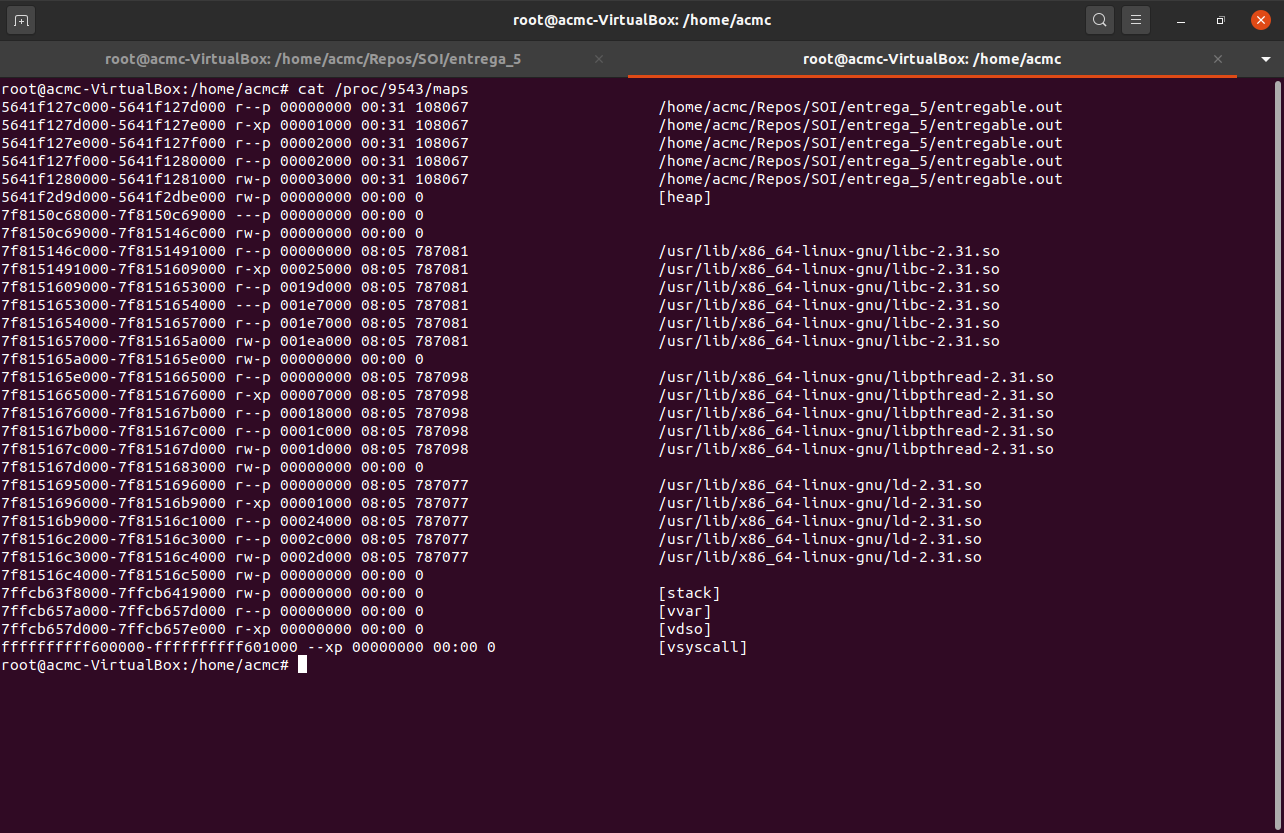
\includegraphics[scale=0.447]{6_hijo1.png}

Esto se corresponde con el stack para el nuevo hilo. En las prácticas optativas pude usar la función {\ttfamily clone()}, que deja ver de forma bastante más expícita la necesidad de crear un stack para el hilo. En el caso de la llamada a {\ttfamily clone()}, primero es necesario reservar manualmente un espacio en la memoria para alojar el stack del nuevo hilo. Esto se hace usando {\ttfamily malloc}, que se encargará de reservar una zona de memoria que aloje el stack. Al llamar a {\ttfamily pthread\_create}, este segmento de memoria se mapea de forma implícita.

En el mapa de memoria, el mapeo de esta entrada es anónimo, porque no se corresponde con ningún archivo, sino que es un segmento que se crea en tiempo de ejecución y sólo está dentro de este proceso.

Si creo el segundo hilo, aparece otro segmento para reservar su stack:

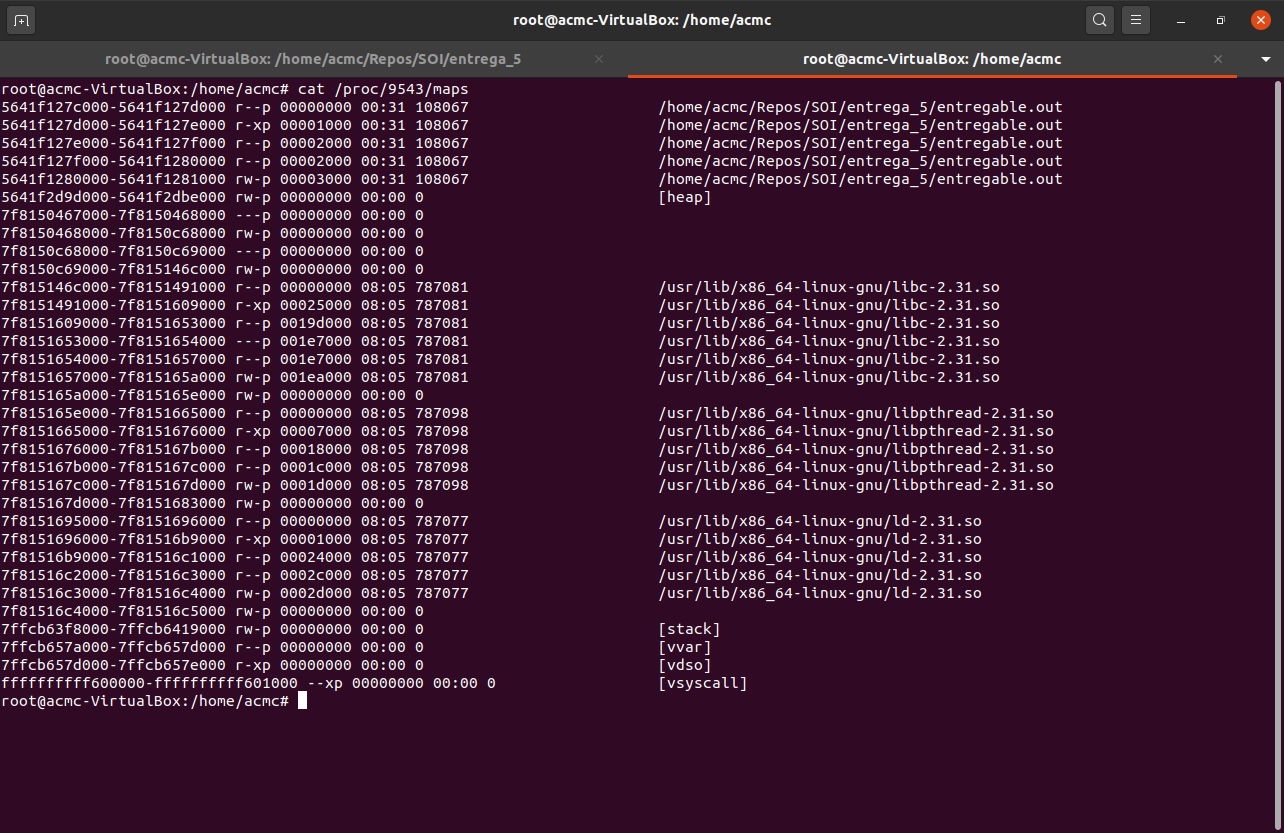
\includegraphics[scale=0.408]{6_hijo2.png}

Las entradas que figuran en el mapa que no tienen ningún tipo de permiso tienen el propósito de servir como protección. Básicamente, están ahí para que, en caso de que intentemos escribir o leer en ellas, tengamos un \emph{segmentation fault} (ya que no deberíamos poder). Esto es lógico si pensamos que el stack puede crecer hasta desbordarse. Si se desborda, en este caso se desbordaría hacia estos segmentos en los que no tenemos permisos, por lo que tendríamos el fallo de segmento que comentaba. Y eso es algo deseable, porque la otra opción sería no tener esos segmentos ``de proteción'' por el medio. En ese caso, podría haber dos situaciones:
\begin{itemize}
    \item Si la memoria no estuviera mapeada, e intentásemos acceder a ella, seguiríamos teniendo un \emph{segmentation fault}, así que en ese caso no cambia nada.
    \item Si resultase que justo de forma contigua al segmento del stack hubiera otro segmento mapeado (por ejemplo, podría ser el stack de otro hilo), ¡podríamos escribir en el stack del otro hilo!
    
    Claramente, esto plantearía un serio problema de protección. Nuestro programa podría sufrir errores gravísimos si algo así sucediera. Por eso es mejor curarnos de males y tener estos segmentos ``de seguridad''. Técnicamente no eliminamos la posibilidad de direccionar a un segmento que no es el deseado, pero si combinamos esta técnica con la de la aleatorización de direcciones, tenemos un ambiente en el que es mucho más difícil que se produzcan esta clase de fallos en la memoria.
\end{itemize}

Me parece muy pertinente volver a hablar aquí de {\ttfamily malloc}, ya que su comportamiento con respecto a la existencia de hilos puede variar según la implementación.

La implementación {\ttfamily dlmalloc}, que es la que se usaba antes en Linux, compartía los segmentos que usaba para la gestión de la memoria dinámica entre todos los hilos. Conceptualmente, este enfoque no plantea ningún problema, ya que el heap se comparte entre los hilos (y también los segmentos anónimos que puede crear {\ttfamily malloc}).

El problema es que esto planteaba problemas de rendimiento. Si dos hilos intentan llamar a {\ttfamily malloc} al mismo tiempo, esta es una carrera crítica, que {\ttfamily malloc} resolvía haciendo una exclusión mutua de la región crítica: primero resolvía una llamada, y una vez resuelta, pasaba a atender la siguiente. De lo contrario, podrían darse problemas de coherencia en los registros internos que usa {\ttfamily malloc}\footnote{\href{https://sploitfun.wordpress.com/2015/02/10/understanding-glibc-malloc/}{Ver más en este enlace}.}.

En cambio, para evitar este problema de rendimiento, la solución que se usa hoy en día es crear nuevos segmentos anónimos para alojar ``\emph{heaps} separados para cada hilo'' (\emph{arenas}). Así, no se pueden producir carreras críticas porque {\ttfamily malloc} accederá al \emph{heap} propio de cada hilo, y ésto permite paralelizar las llamadas a {\ttfamily malloc}. Eso sí, cabe comentar que {\ttfamily malloc} no crea más arenas que el número de cores, ya que no sería eficiente (no se puede llamar paralelamente a {\ttfamily malloc} más veces que el número máximo de hilos que puede haber en un momento determinado). Es decir, existe un límite superior para las arenas.\footnote{Además, es importante señalar que precisamente por este motivo lo que digo de que ``cada hilo'' tiene su propio heap, no es exactamente así. Más bien, se crean tantas arenas como hilos haya, y cuando un hilo solicita memoria a {\ttfamily malloc}, se elige la primera arena que pueda atender la llamada. Un hilo puede tener asignada memoria dinámica en varias arenas.}.

No sale en el código de mi entregable porque no se pide que llame a {\ttfamily malloc}, pero si modifico un poco el código para que los hilos que creo llamen a {\ttfamily malloc}, se puede ver el efecto que comentaba, en el que se crean \emph{arenas} separadas para cada hilo:

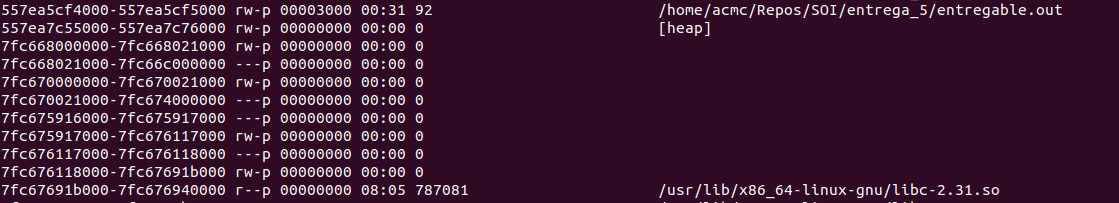
\includegraphics[scale=0.407]{Hilos_con_malloc.png}

Recordemos la imagen anterior en la que veíamos la creación de stacks separados. Pues bien, ahora lo que vemos es, además de que se crean los stacks, que tras llamar a {\ttfamily malloc}, se crean los nuevos segmentos para las arenas. (Aunque liberemos la memoria llamando a {\ttfamily free}, estas áreas anónimas de memoria no se desmapean usando {\ttfamily munmap}, sino que se quedan presentes en el mapa de memoria: podrían ser usadas por otros hilos).

Esto es así porque se usa una implementación distinta, {\ttfamily ptmalloc2}, que se diseñó precisamente como un \emph{fork} de {\ttfamily dlmalloc}, para mejorar su funcionamiento con hilos.

\subsection{Sobre {\ttfamily [vsyscall]}, {\ttfamily [vdso]} y {\ttfamily [vvar]}}

Es curioso comentar la última línea del mapa de memoria, ya que corresponde a una dirección que no está en el espacio de usuario. El espacio de usuario solo llega hasta {\ttfamily 0x7fffffffffff} \footnote{Se puede consultar \href{https://www.kernel.org/doc/Documentation/x86/x86_64/mm.txt}{este enlace} para obtener más detalles al respecto.}. Este segmento aparece reflejado en el mapa de memoria, porque se utilizaba para hacer llamadas al sistema de forma directa \footnote{Hoy en día, solo se mantiene por temas de compatibilidad. En \href{https://lwn.net/Articles/446528/}{este artículo} se comenta en detalle el funcionamiento de esta entrada del mapa.}. También es el uso de {\ttfamily [vdso]}, que se encuentra dentro del espacio de usuario para permitir la aleatoriedad de las direcciones (por los motivos de seguridad que comentaba al principio del informe)\footnote{{\ttfamily [vvar]} complementa la funcionalidad de {\ttfamily [vdso]}. También se comenta en el artículo anterior.}.

\subsection{Enlazado estático y dinámico}

Por defecto, el enlazador de \emph{gcc} utiliza el enlazado dinámico (el caso del mapa de memoria que salía al principio). Esto es porque el enlazado dinámico ofrece varias ventajas, entre las que destaca especialmente el hecho de que reduce considerablemente el tamaño de los ejecutables. Pese a todo, si en vez de compilar el código del entregable de la forma estándar (enlazado dinámico), se compila especificando la opción {\ttfamily -static}, entonces el enlazado será estático, y esto implica que el código de las librerías que incluímos en nuestro programa se incluirá directamente en el código ejecutable. Esto implica un incremento considerable de tamaño (en mi caso, pasé de 17kB a 1,6MB).

En el mapa de memoria, también se verá reflejado dicho cambio:

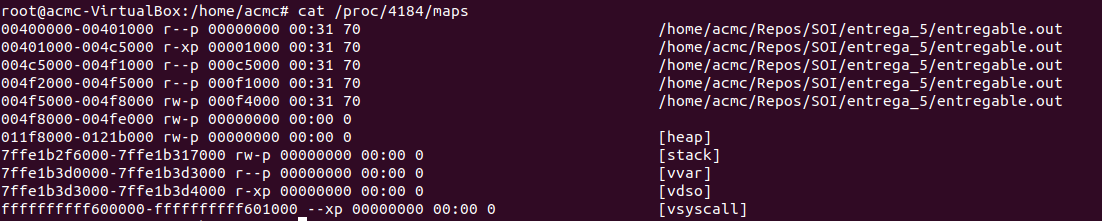
\includegraphics[scale=0.408]{Captura_estatico.png}

Aquí lo que vemos es que su número de entradas ha bajado mucho. Esto es porque todo el código de las librerías, antes se mapeaba en el proceso, y correspondía a las entradas que se mapeaban a {\ttfamily libc-2.31.so}, {\ttfamily libpthread-2.31.so} y {\ttfamily ld-2.31.so}). (Ocupaban varias entradas porque tenían segmentos con diferentes permisos, y también había regiones con permisos {\ttfamily ---p} por el medio por las cuestiones de seguridad que ya mencioné cuando hablé de los hilos).

Ahora, todo el código se carga desde el archivo del ejecutable en sí, por lo que las librerías ya no tienen asignado su propio segmento de memoria, y el número de entradas del mapa baja enormemente (no así el tamaño, como comentaba).

\subsection{{\ttfamily alloca} frente a {\ttfamily malloc}}

En la práctica, se habla también de una función de la familia de {\ttfamily malloc}, {\ttfamily alloca}. Me parece interesante comentar brevemente el funcionamiento de esta última. {\ttfamily alloca}, al contrario que {\ttfamily malloc}, no reserva memoria en el heap o en una región anónima. Lo que hace es decrementar el stack, por lo que nos crea el espacio necesario para almacenar la cantidad solicitada de bytes allí. Si recordamos el apartado en el que hablaba de las variables locales, podremos darnos cuenta de que en el fondo este mecanismo es idéntico al de declarar una variable local en una función. También, como en el caso de las variables locales, al salir de una función, se incrementará el puntero del stack, y por tanto, nuestras variables quedarán ``efectivamente borradas''. (Es decir, podremos reescribir posteriormente en esas posiciones de memoria).

\end{document}